\documentclass[convert = false, tikz]{standalone}
\usepackage[utf8]{inputenc}
\usepackage{tikz}
\usetikzlibrary{automata, positioning, arrows}
 
\usepackage{../../../../style_automata}

% arara: pdflatex
% arara: latexmk: { clean: partial }
\begin{document}
    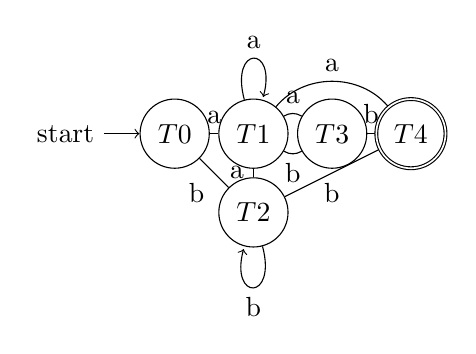
\begin{tikzpicture}
        \node[state, initial] (t0) {$T0$};
        \node[state, right of=t0] (t1) {$T1$};
        \node[state, below of=t1] (t2) {$T2$};
        \node[state, right of=t1] (t3) {$T3$};
        \node[state, accepting, right of=t3] (t4) {$T4$};
	    \draw (t0) edge[above] node{a} (t1)
	    (t0) edge[below left] node{b} (t2)
	    (t1) edge[loop above] node{a} (t1)
	    (t1) edge[below, bend right=30] node{b} (t3)
	    (t2) edge[left] node{a} (t1)
	    (t2) edge[loop below] node{b} (t2)
	    (t3) edge[above, bend right=30] node{a} (t1)
	    (t3) edge[above] node{b} (t4)
	    (t4) edge[above, bend right=50] node{a} (t1)
	    (t4) edge[below] node{b} (t2);
    \end{tikzpicture}
\end{document}
